\documentclass[12pt]{article}

\usepackage{sbc-template}
\usepackage{graphicx,url}
\usepackage[utf8]{inputenc}
\usepackage[T1]{fontenc}
\usepackage{times}
\usepackage{booktabs}

\sloppy

\title{How Much of Traffic Accident Severity Is Predictable\\
from Context? A Leakage Audit on Brazilian Highway Data}

\author{Jo\~ao Pedro Pereira da Luz\inst{1}}

\address{Departamento de Computa\c{c}\~ao -- Universidade Federal do Piau\'i (UFPI)\\
  Teresina -- PI -- Brazil
  \email{joaopedrolluz12@gmail.com}
}

\begin{document}

\maketitle

\begin{abstract}
Can the severity of a road accident be anticipated from where, when and under
which conditions it happens? We frame this question as a supervised
classification task over 342,670 accidents recorded by the Brazilian Federal
Highway Police (PRF) from 2021 to 2025, with models trained on 2021--2023,
tuned on 2024 and tested once on 2025. The same logistic regression and random
forest models are trained on three nested feature sets: context only, context
plus accident dynamics, and a deliberately leaky set with outcome-derived
columns. Context alone reaches a PR-AUC of 0.395 against a no-skill value of
0.283; accident dynamics raise it to 0.528; leaked columns raise it to
0.965--0.994. The context-only model relies mostly on road type and location and
flags 99.0\% of the accidents in Piau\'i as severe, against 54.4\% in the
Southeast.
\end{abstract}

\section{Introduction}

The Brazilian Federal Highway Police (PRF) records tens of thousands of traffic
accidents on federal highways every year and publishes them as open data. In the five years
analysed here, 28.3\% of the recorded accidents left at least one person dead
or seriously injured. These are the cases in which emergency response and
preventive enforcement matter most, which makes accident severity a natural
target for machine learning (ML).

Several recent Brazilian studies train classifiers on PRF data to predict
severity \cite{gabardo2025,mafort2025,fuhr2025}. Their feature sets usually mix
attributes that are known before or at the moment of an accident (location,
time, weather, road layout) with attributes that only exist after someone has
described the event (accident type, cause, number of vehicles and people). The
distinction matters for use: a model meant to guide preventive planning can
only rely on the first group, while the second is available only to triage an
accident that has already been reported. A third group of columns, the victim
counts and the official classification of the accident, is the outcome itself,
and using it as input is a form of data leakage
\cite{kaufman2012,kapoor2023}. Because each study reports a single score for a
single feature set, it is not possible to tell how much of the reported
performance comes from each kind of information.

This work fills that gap. Our research question is: \emph{how much of the
severity of an accident is predictable from context alone, and how much of the
performance obtainable on this dataset depends on information that only exists
after the accident?} We train the same models, with the same hyperparameters
and the same temporal split, on three nested feature sets, and complement the
comparison with robustness checks and an error analysis by region and accident
type. The goal is \emph{predictive, not causal}: we measure which information
helps to anticipate severity, not which factor causes it.

\section{Related Work}

% CONFERIR NOS ORIGINAIS: os detalhes atribuidos a Gabardo et al., Mafort e
% Kappel e Fuhr et al. vieram de resumos e nao da leitura integral dos artigos.

\textbf{Severity prediction on PRF data.} Gabardo et al. \cite{gabardo2025}
classify fatal outcomes in accidents on federal highways of the Brazilian
southern region using PRF data from 2021 to 2024. They compare random forest,
$k$-nearest neighbours and a multilayer perceptron, balance the classes with
SMOTE and use SHAP to analyse feature influence, reporting an AUC-ROC of 0.99
for random forest and $k$-nearest neighbours. Mafort and Kappel
\cite{mafort2025} study accidents on federal highways in the state of Rio de
Janeiro from 2020 to 2023 with several classifiers and report a random forest
with 86\% accuracy and an F1-score of 59\% when vehicle and environment
attributes are used.

\textbf{Data quality.} F\"uhr et al. \cite{fuhr2025} focus on accidents on the
BR-101 in Santa Catarina. They identify inconsistencies in PRF records and
compare random forest, support vector machine and multilayer perceptron models
trained on the original and on the improved data, showing that the preparation
of these records affects the results.

\textbf{Leakage and evaluation on imbalanced data.} Kaufman et al.
\cite{kaufman2012} define leakage as the use of information that would not be
legitimately available at prediction time, and Kapoor and Narayanan
\cite{kapoor2023} show that it is a widespread cause of over-optimistic results
in applied ML. Saito and Rehmsmeier \cite{saito2015} show that the
precision--recall curve is more informative than the ROC curve when the
positive class is rare. A pair such as 86\% accuracy and 59\% F1 illustrates
the point: on an imbalanced target, accuracy alone says little.

Our work differs from the PRF studies in three ways: (i) it covers the whole
country, which allows checking whether a model behaves equally across regions;
(ii) it uses a temporal split instead of a random one; and (iii) its main
contribution is a comparison between feature sets defined by the moment at
which each feature becomes available, rather than a single model.

\section{Methodology}

\subsection{Data acquisition and sample}

All data are open government data published by the PRF, one file per year,
with accidents grouped by occurrence \cite{prf2026}. The files require no registration and are downloaded
directly by the notebook. The unit of analysis is one accident, described by
30 attributes. An accident is labelled \emph{severe} if it has at least one
death or one seriously injured person, and \emph{non-severe} otherwise. The
data were split by year, as shown in Table~\ref{tab:sample}. The share of
severe accidents is practically the same in every set, so differences in
performance between sets cannot be attributed to a change in the base rate.

\begin{table}[ht]
\centering
\caption{Data split and share of severe accidents.}
\label{tab:sample}
\begin{tabular}{llrr}
\toprule
Set & Years & Accidents & Severe \\
\midrule
Training   & 2021--2023 & 196,939 & 28.3\% \\
Validation & 2024       &  73,202 & 28.2\% \\
Test       & 2025       &  72,529 & 28.3\% \\
\midrule
Total      & 2021--2025 & \textbf{342,670} & 28.3\% \\
\bottomrule
\end{tabular}
\end{table}

Quality checks found no duplicated rows or identifiers, complete coverage of
each year from January 1 to December 31, and no inconsistency among the victim
counts that define the label. Two problems were found in other columns: in
5.4\% of the accidents the number of people involved differs from the sum of
its categories, which affects only feature sets B and C below, and about 20\%
of the records have a time on the exact hour, against 1.7\% expected, so the
recorded time is often an estimate. The only missing values are in the official
classification (5 rows) and in administrative columns that are not used, so no
row was discarded. Categories such as ``Ignored'' were kept as categories. The
way the form is filled also changed: the share of records with more than one
value in the road-layout field rose from about 10\% in 2021--2022 to about 25\%
from 2023 onwards.

\subsection{Features}

To keep validation and test data out of every decision, the exploratory
analysis that guided the feature design used the training years only.
Row-wise transformations were applied before splitting: hour of day also
encoded as sine and cosine, month, a weekend indicator, an urban-area indicator
and the multi-valued road-layout field expanded into 12 binary indicators. The
features are grouped into three nested sets:

\begin{itemize}
\item \textbf{(A) Context, 28 features:} time (hour, month, weekday, day
phase), location (state, highway, kilometre, coordinates, direction), weather,
road type, road layout and urban area. Known before or at the moment of the
accident.
\item \textbf{(B) Context + dynamics, 32 features:} A plus accident type,
accident cause, number of vehicles and number of people involved. Known only
after the accident has been described.
\item \textbf{(C) With leakage, 36 features:} B plus the official
classification of the accident and the counts of slightly injured, unharmed
and unknown-status people. Known only once the outcome is known; used solely
to measure the effect of leakage.
\end{itemize}

\subsection{Experimental protocol and models}

We train on 2021--2023, choose hyperparameters and the decision threshold on
2024, and test once on 2025. This temporal split mimics the real use of the
model, in which a model trained on the past is applied to future accidents.
Standardisation of numeric features and one-hot encoding of categorical
features (grouping categories with fewer than 50 occurrences) are fitted inside
a scikit-learn pipeline \cite{pedregosa2011} on the training set only, so they
never see validation or test data.

We compare four models: (i) a baseline that always predicts the majority
class; (ii) a baseline that always predicts the severe class; (iii) a logistic
regression; and (iv) a random forest \cite{breiman2001}, the algorithm most
used in the related work, which can capture interactions among features. Both
learned models use class weights inversely proportional to class frequency
instead of synthetic oversampling. A small grid search on set A selected
$C = 0.1$ for the logistic regression and, for the random forest, 100 trees
with unlimited depth, at least 20 samples per leaf and each tree trained on
half of the training rows. The same hyperparameters were reused for sets B and
C, so that only the features change between scenarios.

Since only 28.3\% of the test accidents are severe, accuracy would be
misleading. The main metric is the area under the precision--recall curve
(PR-AUC), whose no-skill value equals the positive rate, 0.283
\cite{saito2015}. We also report ROC-AUC and, at the threshold that maximises
F1 on the validation year, F1, precision, recall and accuracy. 95\% confidence
intervals are obtained by bootstrapping the test set (500 resamples).
Robustness is assessed by repeating the experiment with a stratified random
split over the same rows and by training the random forest with three seeds.
Feature relevance is measured by permutation importance on the validation year.

\section{Results and Discussion}

\subsection{Overall performance}

Table~\ref{tab:main} summarises the results on the 2025 test set for the
context features. Both learned models beat the baselines, but by a small
margin: the random forest reaches a PR-AUC of 0.395 against the no-skill value
of 0.283, and a ROC-AUC of 0.627. At the F1-maximising threshold it recovers
78.3\% of the severe accidents, but does so by flagging 67.0\% of all
accidents; its F1 of 0.465 is only slightly above the 0.441 obtained by
labelling every accident as severe. Used as a ranking, the gain is modest:
among the 10\% of accidents with the highest predicted risk, 46.9\% are severe,
1.7 times the base rate. The table also shows why accuracy is misleading here:
the highest accuracy (0.717) belongs to the baseline that detects no severe
accident at all.

\begin{table}[ht]
\centering
\caption{Performance on the 2025 test set, context features only (set A).
Models trained on 2021--2023, threshold chosen on 2024. No-skill PR-AUC: 0.283.}
\label{tab:main}
\small
\begin{tabular}{lcccccc}
\toprule
Model & PR-AUC [95\% CI] & ROC-AUC & F1 & Prec. & Recall & Acc. \\
\midrule
Always non-severe   & 0.283                & 0.500 & 0.000 & 0.000 & 0.000 & 0.717 \\
Always severe       & 0.283                & 0.500 & 0.441 & 0.283 & 1.000 & 0.283 \\
Logistic regression & 0.386 [0.380, 0.392] & 0.620 & 0.460 & 0.321 & 0.810 & 0.463 \\
Random forest       & 0.395 [0.389, 0.401] & 0.627 & 0.465 & 0.331 & 0.783 & 0.491 \\
\bottomrule
\end{tabular}
\end{table}

The grid search points to the probable cause of the weak result. Validation
PR-AUC varied only between 0.400 and 0.404 across random forest configurations
and stayed at 0.397 for every regularisation strength of the logistic
regression, which suggests that the limit lies in the information available in
the features rather than in model capacity. Variables that plausibly drive
severity, such as speed, seat-belt use and vehicle type, are absent from the
occurrence-level data.

\subsection{Which feature set carries the information?}

Figure~\ref{fig:sets} answers the research question. Adding accident dynamics
(set B) raises the random forest PR-AUC from 0.395 to 0.528 and the ROC-AUC
from 0.627 to 0.714: knowing \emph{how} the accident happened says more about
severity than all context features together. This is consistent with the
exploratory analysis of the training years, in which 68.0\% of pedestrian
collisions and 62.8\% of head-on collisions are severe, against 33.7\% on
single carriageways, the road-type category with the highest share. These
attributes, however, only exist after the accident.

\begin{figure}[ht]
\centering
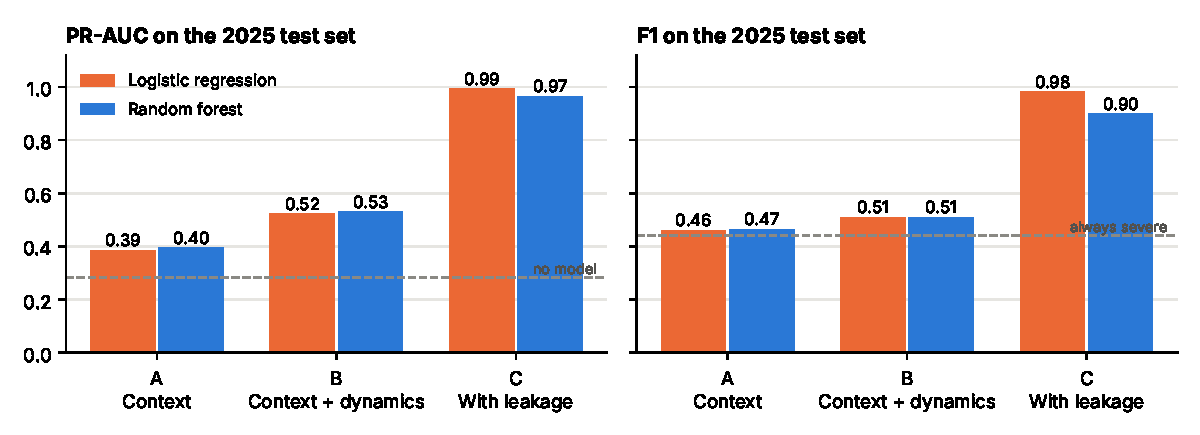
\includegraphics[width=\textwidth]{figuras/fig_feature_sets.pdf}
\caption{PR-AUC and F1 on the 2025 test set for the three feature sets. Dashed
lines show the no-skill PR-AUC and the F1 of always predicting severe.}
\label{fig:sets}
\end{figure}

With outcome-derived columns (set C) the PR-AUC jumps to 0.965 for the random
forest and 0.994 for the logistic regression, with F1 up to 0.982. This is not
model quality: the added columns are the ones from which the label is
computed, and when they are filled in the outcome is already known. Logistic
regression outperforms the random forest in this scenario, probably because
the leaked relation is close to a direct rule on a few columns, which a linear
model captures immediately, while each tree split only sees a random subset of
the features.

The practical implication is that a score on this dataset cannot be
interpreted without knowing which columns were used and when each becomes
available: on the same data and with the same models, PR-AUC ranges from 0.40
to 0.99 depending only on the feature set. Our set B, the closest to the
feature sets of the related work, yields an F1 of 0.51, the same order of
magnitude as the 59\% reported by Mafort and Kappel \cite{mafort2025}. A
direct numerical comparison is not possible, because targets, regions and
periods differ.

\subsection{Robustness}

Replacing the temporal split by a stratified random split over the same rows
changed PR-AUC by at most 0.005 (0.395 versus 0.400 for the random forest). We
expected the random split to inflate the results, given the change in how
records are filled; the data do not support this hypothesis, and we report it
as a negative result: the relation between context and severity was stable
from 2021 to 2025. Across three seeds, the standard deviation of the random
forest PR-AUC was 0.0001. The 95\% bootstrap interval for the PR-AUC
difference between random forest and logistic regression is 0.007 to 0.012:
the random forest is consistently better, but by a margin of little practical
relevance, while the logistic regression trains in a few seconds.

\subsection{Does performance change across regions?}

In the training years, the share of severe accidents differs strongly across
the country, from about 19\% in S\~ao Paulo to more than 40\% in Piau\'i,
Par\'a and Maranh\~ao (Figure~\ref{fig:uf}). Permutation importance shows that
the context-only random forest relies mostly on road type (a PR-AUC drop of
0.027 when shuffled) and on location features (0.019 for latitude), while
weather and road layout have an effect close to zero.

\begin{figure}[ht]
\centering
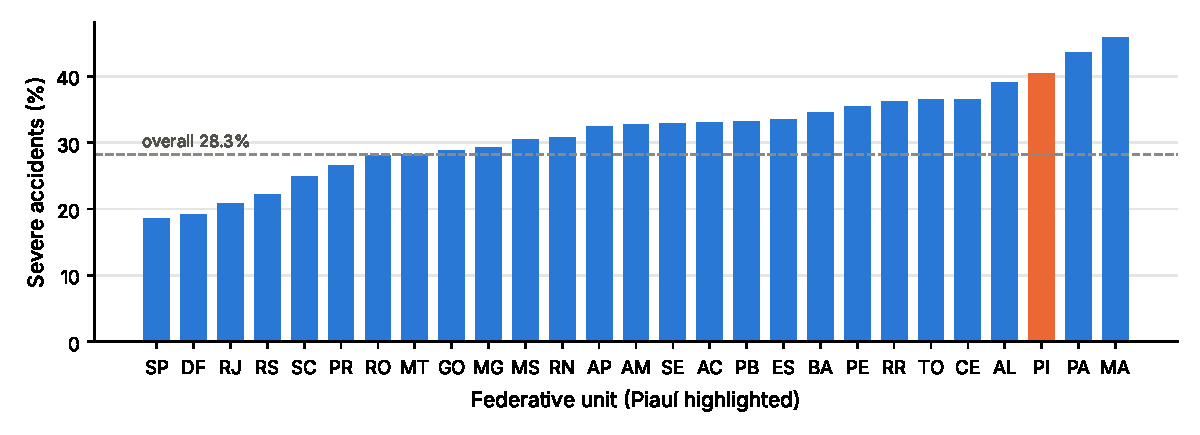
\includegraphics[width=\textwidth]{figuras/fig_uf.pdf}
\caption{Share of severe accidents by federative unit in the training years
(2021--2023). The dashed line shows the overall share.}
\label{fig:uf}
\end{figure}

As a consequence, the model behaves very differently across regions
(Figure~\ref{fig:regions}). With a single national threshold it flags 99.0\% of
the accidents in Piau\'i, 90.6\% in the North and 88.8\% in the Northeast as
severe, against 54.4\% in the Southeast and 56.1\% in the South. The recall
close to 100\% in Piau\'i is therefore not evidence of good performance. Within
each region the PR-AUC is only 1.2 to 1.4 times the regional base rate, and the
ROC-AUC drops to 0.58 in the Central-West: part of the national performance
comes from telling regions apart, not accidents.

\begin{figure}[ht]
\centering
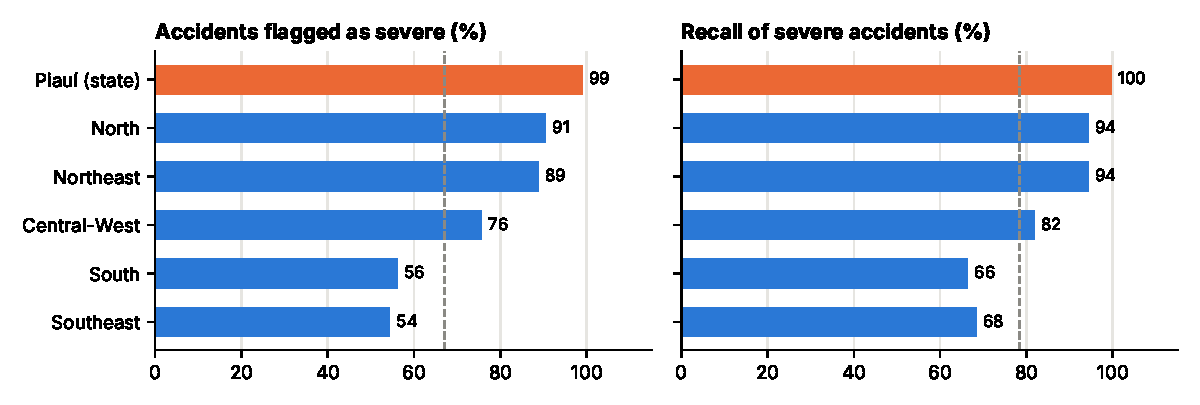
\includegraphics[width=\textwidth]{figuras/fig_regions.pdf}
\caption{Share of accidents flagged as severe and recall of severe accidents by
region on the 2025 test set, context-only random forest. Dashed lines show the
national values.}
\label{fig:regions}
\end{figure}

\subsection{Error analysis, limitations and risks}

Crossing the errors with the accident type, which the context-only model does
not see, shows what it misses. It detects 94\% of the severe head-on
collisions but only 69\% of the severe rear-end collisions and 63\% of the
severe same-direction side collisions. Among the severe accidents that were
missed, only 14.0\% happened on single carriageways (68.4\% among the detected
ones) and 16.1\% at night (45.7\%). The model has essentially learned the
pattern ``single carriageway, at night, outside urban areas''; severe accidents
outside this pattern are the ones it loses.

The study has important limitations. (i) It is predictive and does not identify
causal effects. (ii) The dataset only contains accidents that happened and were
recorded, so the model estimates severity given an accident, not the chance of
one; this explains why, in the training years, accidents under rain have a
lower share of severe outcomes (24.3\%) than under clear sky (29.5\%), probably
because rain produces many minor accidents. (iii) Under-reporting of minor
accidents may differ across regions, in which case part of the regional
difference would be an artefact of data collection that the model would
reproduce. (iv) The label merges deaths and serious injuries, and the
``seriously injured'' status is assigned by the officer at the scene. (v) Only
two algorithms and a small hyperparameter grid were evaluated, and the tested
model was not refitted on the validation year. (vi) The predicted
probabilities are not calibrated: among accidents scored around 0.45, only
26\% are severe, a consequence of class weighting.

Regarding risks, the context-only model must not support decisions about
individual occurrences: it would prioritise almost every accident in the North
and Northeast and miss about one third of the severe accidents in the South and
Southeast. A defensible use is aggregate, indicating combinations of road type,
highway stretch and time of day with a higher share of severe outcomes, always
together with accident counts.

\section{Conclusion}

We audited where the predictive signal comes from when classifying accident
severity on PRF open data. With 342,670 accidents from 2021 to 2025 and a
temporal evaluation, context alone proved weakly predictive (PR-AUC 0.395
against 0.283 without a model); information about the accident dynamics added
substantially (0.528); and outcome-derived columns produced near-perfect and
practically useless scores (0.965--0.994). Answering the research question: on
this dataset the choice of features matters far more than the choice of
algorithm or split strategy, accuracy hides the problem, and a model with a
reasonable national average can behave as an ``always severe'' rule in a whole
state.

Future work includes using the person-level and vehicle-level PRF data to add
the profile of the people and vehicles involved, training or thresholding
models by region, calibrating the predicted probabilities, and aggregating
accidents by highway stretch together with traffic volume to estimate the rate
of severe accidents per kilometre.

\section*{Data and Code Availability}

The data are public, and the notebook downloads them directly from the PRF
open data portal (section ``Acidentes'', files grouped by occurrence, 2021 to
2025). The notebook, the figures and the source of this paper are in a public
repository, and the notebook runs end-to-end in Google Colab with no local
files:
% Se preferir, troque o link do notebook pelo link de compartilhamento do Colab no seu Google Drive.
\begin{itemize}\raggedright
\item Data: \url{https://www.gov.br/prf/pt-br/acesso-a-informacao/dados-abertos/dados-abertos-da-prf}
\item Repository: \url{https://github.com/JoaoPedroLuz12/Clauduxo}
\item Notebook (Google Colab): \url{https://colab.research.google.com/github/JoaoPedroLuz12/Clauduxo/blob/claude/wizardly-brown-olt8sr/notebook/acidentes_prf_gravidade.ipynb}
\end{itemize}

\section*{Use of Large Language Models}

% AJUSTAR se algo abaixo nao corresponder ao que voce fez.
This work used Claude (Anthropic), through Claude Code, as an assistant. It was
used to: break down the assignment into steps; propose candidate application
areas and public datasets; search for related literature; design the
experimental protocol; generate, explain and debug the notebook code; and draft
this paper in English. The author chose the application area (road safety)
among the options proposed, approved the problem formulation and the
evaluation plan, and directed the work with requests such as \emph{``Look at
what the professor asks and build a path of what must be done to get the
maximum grade''}, \emph{``Can I simulate an accident and have the machine tell
me how severe it is?''} and \emph{``Does the professor ask for what is being
done, or did you just do what you thought was best?''} (translated from
Portuguese). The outputs were verified as follows: the notebook was executed
end-to-end in Google Colab without errors, and its outputs were compared with
a second run in an environment with the same library versions; every number in
this paper was checked against the notebook outputs; and the download links of
the data were tested.
% ACRESCENTAR depois de fazer: "every reference was checked against its
% original source" e "the author reviewed all text and results".
The author is responsible for the content.

\bibliographystyle{sbc}
\bibliography{refs}

\end{document}
